\documentclass{article}
\usepackage{polski}
\usepackage{float}
\usepackage{adjustbox}
\usepackage{tikz}
\usepackage{graphicx}
\graphicspath{ {./latexImages/} }

\title{Sprawozdanie 1 - Algorytmy Optymalizacji Dyskretnej}
\author{Michał Kallas}
\date{Październik 2024}

\begin{document}

\maketitle

\section{Zadanie 1}
\subsection{Opis i rozwiązanie}
W zadaniu należało zaimplementować algorymty BFS i DFS z możliwością wyświetlania kolejności przejścia po grafie oraz
drzew przeszukań.

Zaimplementowałem iteracyjne wersje tych algorytmów z kolejką i stosem. Ich złożoność to $O(|V| + |E|)$.

\subsection{Grafy}
\begin{figure}[H]
\centering
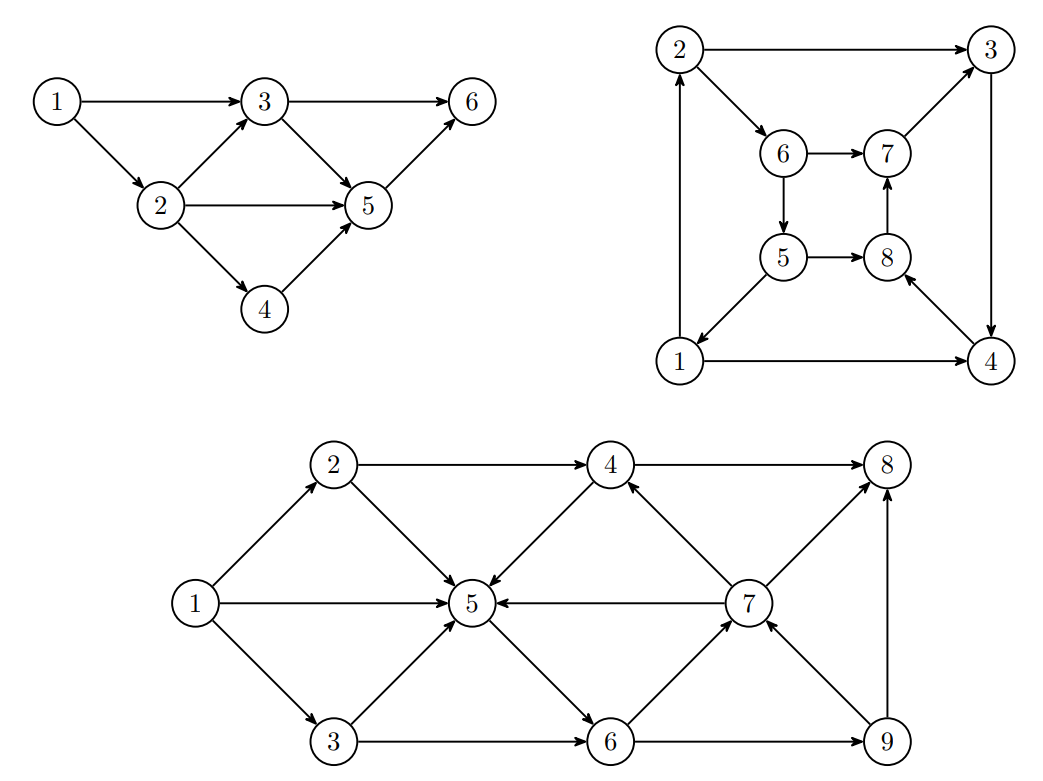
\includegraphics[scale=0.4]{testGraphs}
\caption{Grafy testowe z polecenia, numerowane od 1 do 3 od lewej do prawej.}
\end{figure}

\begin{figure}[H]
\centering
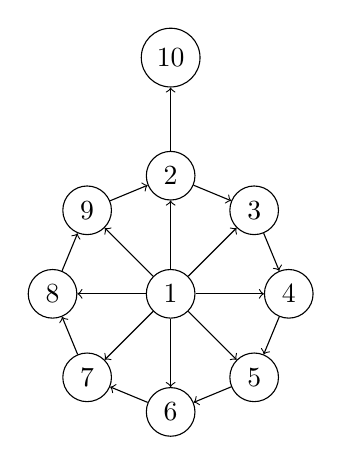
\begin{tikzpicture}[node distance={15mm}, main/.style = {draw, circle}] 
\node[main] (1) {1};
\node[main] (2) [above of=1] {2};
\node[main] (10) [above of=2] {10};
\node[main] (3) [above right of=1] {3};
\node[main] (4) [right of=1] {4};
\node[main] (5) [below right of=1] {5};
\node[main] (6) [below of=1] {6};
\node[main] (7) [below left of=1] {7};
\node[main] (8) [left of=1] {8};
\node[main] (9) [above left of=1] {9};
\draw[->] (2) -- (3);
\draw[->] (2) -- (10);
\draw[->] (3) -- (4);
\draw[->] (4) -- (5);
\draw[->] (5) -- (6);
\draw[->] (6) -- (7);
\draw[->] (7) -- (8);
\draw[->] (8) -- (9);
\draw[->] (9) -- (2);
\draw[->] (1) -- (2);
\draw[->] (1) -- (3);
\draw[->] (1) -- (4);
\draw[->] (1) -- (5);
\draw[->] (1) -- (6);
\draw[->] (1) -- (7);
\draw[->] (1) -- (8);
\draw[->] (1) -- (9);
\end{tikzpicture}
\caption{Mój graf testowy - graf nr 4.}
\end{figure}

\subsection{Wyniki}
\begin{table}[H]
\begin{adjustbox}{center}
\begin{tabular}{|c|c|c|c|}
    \hline
    Graf & Skierowany & Kolejność BFS & Kolejność DFS\\
    \hline
    1 & NIE & [1 3 2 5 6 4] & [1 2 4 5 6 3]\\
    \hline
    2 & NIE & [1 2 4 5 3 6 8 7] & [1 5 6 7 8 4 3 2]\\
    \hline
    3 & NIE & [1 2 3 5 4 6 7 8 9] & [1 5 7 9 8 4 2 6 3]\\
    \hline
    4 & NIE & [1 2 3 4 5 6 7 8 9 10] & [1 9 2 3 4 5 6 7 8 10]\\
    \hline
    1 & TAK & [1 3 2 5 6 4] & [1 2 4 5 6 3]\\
    \hline
    2 & TAK & [1 2 4 3 6 8 5 7] & [1 4 8 7 3 2 6 5]\\
    \hline
    3 & TAK & [1 2 3 5 4 6 8 7 9] & [1 5 6 9 8 7 4 3 2]\\
    \hline
    4 & TAK & [1 2 3 4 5 6 7 8 9 10] & [1 9 2 3 4 5 6 7 8 10]\\
    \hline
\end{tabular}
\end{adjustbox}
\caption{Porównanie kolejności przechodzenia wierzchołków przez BFS i DFS.}
\end{table}

\subsection{Grafy}

\begin{figure}[H]
\begin{minipage}{0.45\textwidth} % Left side
  \centering
  \begin{tikzpicture}
    \node {1}
      child { node {3}
        child { node {5} }
        child { node {6} }
      }
      child { node {2}
        child { node {4} }
      };
  \end{tikzpicture}
\end{minipage}
\hfill
\begin{minipage}{0.45\textwidth} % Right side
  \centering
  \begin{tikzpicture}
    \node {1}
      child { node {2}
        child { node {4}
          child { node {5}
            child { node {6} }
          }
        }
        child { node {3} }
      };
  \end{tikzpicture}
\end{minipage}
\caption{Drzewo przeszukań BFS(po lewej) oraz DFS(po prawej) dla pierwszego grafu skierowanego.}
\end{figure}

\begin{figure}[H]
\centering
  \begin{tikzpicture}
    \node {1}
      child { node {2}
        child { node {10} }
      }
      child { node {3} }
      child { node {4} }
      child { node {5} }
      child { node {6} }
      child { node {7} }
      child { node {8} }
      child { node {9} };
  \end{tikzpicture}
\hfill
  \begin{tikzpicture}
    \node {1}
      child { node {9}
        child { node {2}
          child { node {3}
            child { node {4}
              child { node {5}
                child { node {6}
                  child { node {7}
                    child { node {8} }
                  }
                }
              }
            }
          }
        }
        child { node {10} }
      };
  \end{tikzpicture}
\caption{Drzewo przeszukań BFS(u góry) oraz DFS(na dole) dla mojego grafu skierowanego.}
\end{figure}

\subsection{Czasy}
\begin{table}[H]
\begin{adjustbox}{center}
\begin{tabular}{|c|c|c|c|c|c|}
    \hline
    Graf & Skierowany & $|V|$ & $|E|$ & Czas BFS [ns] & Czas DFS [ns]\\
    \hline
    1 & NIE & 6 & 9 & 5500 & 4200\\
    \hline
    2 & NIE & 8 & 12 & 2900 & 4400\\
    \hline
    3 & NIE & 9 & 17 & 3200 & 5900\\
    \hline
    1 & TAK & 6 & 9 & 1800 & 2200\\
    \hline
    2 & TAK & 8 & 12 & 2300 & 2600\\
    \hline
    3 & TAK & 9 & 17 & 2300 & 3200\\
    \hline
\end{tabular}
\end{adjustbox}
\caption{Porównanie czasów wykonania BFS i DFS dla testowych grafów.}
\end{table}


\section{Zadanie 2}
\subsection{Opis i rozwiązanie}
W zadaniu należało zaimplementować sortowanie topologiczne z możliwością wyświetlenia wierzchołków w posortowanej
kolejności.

Zastosowałem tutaj algorytm Kahna. Jego złożoność to $O(|V| + |E|)$.
\subsection{Grafy}

\begin{figure}[H]
\centering
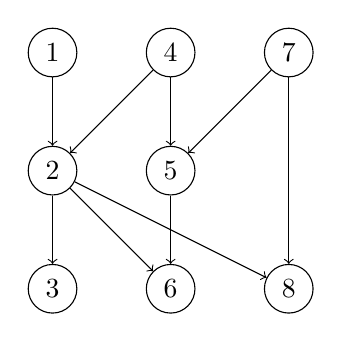
\begin{tikzpicture}[node distance={15mm}, main/.style = {draw, circle}] 
\node[main] (1) {1};
\node[main] (2) [below of=1] {2};
\node[main] (3) [below of=2] {3};
\node[main] (4) [right of=1] {4};
\node[main] (5) [right of=2] {5};
\node[main] (6) [right of=3] {6};
\node[main] (7) [right of=4] {7};
\node[main] (8) [right of=6] {8};
\draw[->] (1) -- (2);
\draw[->] (2) -- (3);
\draw[->] (2) -- (6);
\draw[->] (2) -- (8);
\draw[->] (4) -- (2);
\draw[->] (4) -- (5);
\draw[->] (5) -- (6);
\draw[->] (7) -- (5);
\draw[->] (7) -- (8);
\end{tikzpicture}
\caption{Skierowany graf bez cyklu.}
\end{figure}

\begin{figure}[H]
\centering
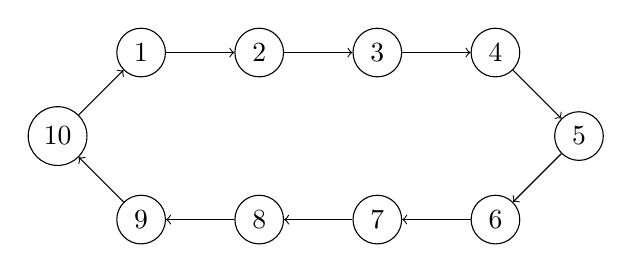
\begin{tikzpicture}[node distance={15mm}, main/.style = {draw, circle}] 
\node[main] (1) {1};
\node[main] (2) [right of=1] {2};
\node[main] (3) [right of=2] {3};
\node[main] (4) [right of=3] {4};
\node[main] (5) [below right of=4] {5};
\node[main] (6) [below left of=5] {6};
\node[main] (7) [left of=6] {7};
\node[main] (8) [left of=7] {8};
\node[main] (9) [left of=8] {9};
\node[main] (10) [below left of=1] {10};
\draw[->] (1) -- (2);
\draw[->] (2) -- (3);
\draw[->] (3) -- (4);
\draw[->] (4) -- (5);
\draw[->] (5) -- (6);
\draw[->] (6) -- (7);
\draw[->] (7) -- (8);
\draw[->] (8) -- (9);
\draw[->] (9) -- (10);
\draw[->] (10) -- (1);
\end{tikzpicture}
\caption{Skierowany graf z cyklem.}
\end{figure}

\subsection{Wyniki}
\begin{table}[H]
\begin{adjustbox}{center}
\begin{tabular}{|c|c|}
    \hline
    Graf & Wynik Sortowania topologicznego\\
    \hline
    1 & [1 4 7 2 5 8 3 6 ]\\
    \hline
    2 & Graf posiada cykl\\
    \hline
\end{tabular}
\end{adjustbox}
\caption{Porównanie wyników sortowania topologicznego dla grafu acyklicznego i cyklicznego przez algorytm Kahna.}
\end{table}


\subsection{Czasy}
\begin{table}[H]
\begin{adjustbox}{center}
\begin{tabular}{|c|c|c|c|c|}
    \hline
    Plik & Acykliczny & $|V|$ & $|E|$ & Czas [ns]\\
    \hline
    \textit{g2a-1.txt} & TAK & 16 & 33 & 18700\\
    \hline
    \textit{g2a-2.txt} & TAK & 100 & 261 & 22500\\
    \hline
    \textit{g2a-3.txt} & TAK & 1600 & 4641 & 362900\\
    \hline
    \textit{g2a-4.txt} & TAK & 10000 & 29601 & 1745499\\
    \hline
    \textit{g2a-5.txt} & TAK & 160000 & 478401 & 30075586\\
    \hline
    \textit{g2a-6.txt} & TAK & 1000000 & 2996001 & 215613800\\
    \hline
    \textit{g2b-1.txt} & NIE & 16 & 34 & 6000\\
    \hline
    \textit{g2b-2.txt} & NIE & 100 & 262 & 27800\\
    \hline
    \textit{g2b-3.txt} & NIE & 1600 & 4642 & 240600\\
    \hline
    \textit{g2b-4.txt} & NIE & 10000 & 29602 & 1352600\\
    \hline
    \textit{g2b-5.txt} & NIE & 160000 & 478402 & 21810148\\
    \hline
    \textit{g2b-6.txt} & NIE & 1000000 & 2996002 & 164590632\\
    \hline
\end{tabular}
\end{adjustbox}
\caption{Porównanie czasów wykonania sortowania topologicznego algorytmem Kahna dla danych z plików testowych.}
\end{table}

\section{Zadanie 3}
\subsection{Opis i rozwiązanie}
W zadaniu należało zaimplementować algorytm zwracający rozkład grafu na silnie spójne składowe. Powinien także
wypisywać ich ilość oraz ilość wierzchołków w każdej z nich.

Skorzystałem tutaj z algorytmu Tarjana o złożoności $O(|V| + |E|)$.

\subsection{Grafy}
\begin{figure}[H]
\centering
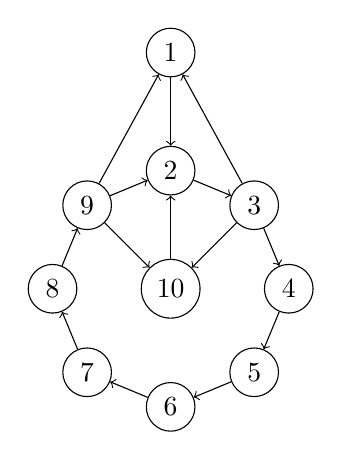
\begin{tikzpicture}[node distance={15mm}, main/.style = {draw, circle}] 
\node[main] (10) {10};
\node[main] (2) [above of=10] {2};
\node[main] (1) [above of=2] {1};
\node[main] (3) [above right of=10] {3};
\node[main] (4) [right of=10] {4};
\node[main] (5) [below right of=10] {5};
\node[main] (6) [below of=10] {6};
\node[main] (7) [below left of=10] {7};
\node[main] (8) [left of=10] {8};
\node[main] (9) [above left of=10] {9};
\draw[->] (1) -- (2);
\draw[->] (2) -- (3);
\draw[->] (3) -- (4);
\draw[->] (3) -- (1);
\draw[->] (3) -- (10);
\draw[->] (4) -- (5);
\draw[->] (5) -- (6);
\draw[->] (6) -- (7);
\draw[->] (7) -- (8);
\draw[->] (8) -- (9);
\draw[->] (9) -- (2);
\draw[->] (9) -- (1);
\draw[->] (9) -- (10);
\draw[->] (10) -- (2);
\end{tikzpicture}
\caption{Graf silnie spójny.}
\end{figure}

\begin{figure}[H]
\centering
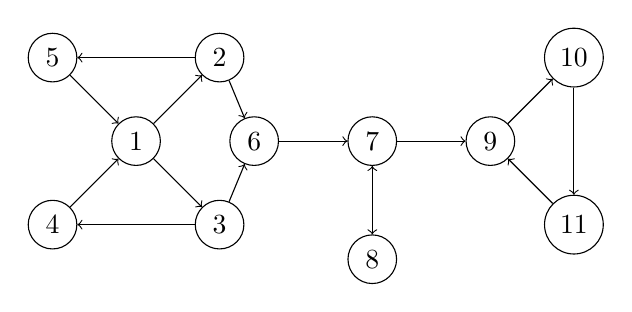
\begin{tikzpicture}[node distance={15mm}, main/.style = {draw, circle}] 
\node[main] (1) {1};
\node[main] (2) [above right of=1] {2};
\node[main] (3) [below right of=1] {3};
\node[main] (4) [below left of=1] {4};
\node[main] (5) [above left of=1] {5};
\node[main] (6) [right of=1] {6};
\node[main] (7) [right of=6] {7};
\node[main] (8) [below of=7] {8};
\node[main] (9) [right of=7] {9};
\node[main] (10) [above right of=9] {10};
\node[main] (11) [below right of=9] {11};
\draw[->] (1) -- (2);
\draw[->] (1) -- (3);
\draw[->] (2) -- (5);
\draw[->] (2) -- (6);
\draw[->] (3) -- (4);
\draw[->] (3) -- (6);
\draw[->] (4) -- (1);
\draw[->] (5) -- (1);
\draw[->] (6) -- (7);
\draw[->] (7) -- (8);
\draw[->] (7) -- (9);
\draw[->] (8) -- (7);
\draw[->] (9) -- (10);
\draw[->] (10) -- (11);
\draw[->] (11) -- (9);
\end{tikzpicture}
\caption{Graf z 4 silnie spójnymi składowymi.}
\end{figure}


\subsection{Wyniki}
\begin{table}[H]
\begin{adjustbox}{center}
\begin{tabular}{|c|c|c|}
    \hline
    Graf & Ilość silnie spójnych składowych & Silnie spójne składowe\\
    \hline
    1 & 1 & [10 9 8 7 6 5 4 3 2 1]\\
    \hline
    2 & 4 & [11 10 9], [8 7], [6], [4 3 5 2 1]\\
    \hline
\end{tabular}
\end{adjustbox}
\caption{Porównanie podziału na silnie spójne składowe przez algorytm Tarjana.}
\end{table}

\subsection{Czasy}
\begin{table}[H]
\begin{adjustbox}{center}
\begin{tabular}{|c|c|c|c|}
    \hline
    Plik & $|V|$ & $|E|$ & Czas [ns]\\
    \hline
    \textit{g3-1.txt} & 16 & 39 & 11275\\
    \hline
    \textit{g3-2.txt} & 107 & 185 & 31808\\
    \hline
    \textit{g3-3.txt} & 1008 & 1609 & 202491\\
    \hline
    \textit{g3-4.txt} & 10009 & 15943 & 3995289\\
    \hline
    \textit{g3-5.txt} & 100010 & 159679 & 20828123\\
    \hline
    \textit{g3-6.txt} & 1000011 & 1598897 & 230059301\\
    \hline
\end{tabular}
\end{adjustbox}
\caption{Porównanie czasów znalezienia silnie spójnych składowych algorytmem Tarjana dla danych z plików testowych.}
\end{table}

\section{Zadanie 4}
\subsection{Opis i rozwiązanie}
W zadaniu należało zaimplementować algorytm sprawdzający czy graf jest dwudzielny. Powinien wypisywać rozbicie grafu
na 2 zbiory wierzchołków, jeśli tak jest.

Skorzystałem tutaj ze zmodyfikowanej wersji BFSa, która koloruje wierzchołki na dwa kolory. Jeśli graf można
pokolorować w taki sposób, żeby sąsiednie wierzchołki nie miały tego samego koloru, to znaczy, że graf jest dwudzielny.
Złożoność tego algorytmu to $O(|V| + |E|)$.

\subsection{Grafy}

\begin{figure}[H]
\centering
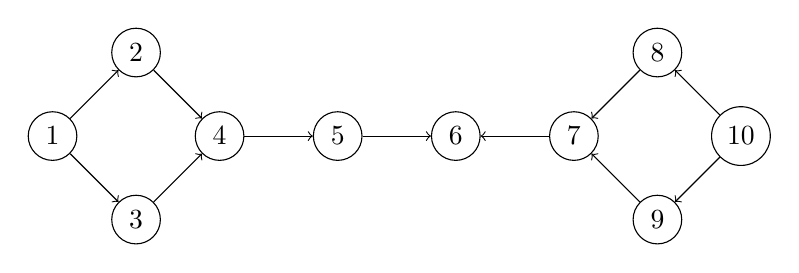
\begin{tikzpicture}[node distance={15mm}, main/.style = {draw, circle}] 
\node[main] (1) {1};
\node[main] (2) [above right of=1] {2};
\node[main] (3) [below right of=1] {3};
\node[main] (4) [below right of=2] {4};
\node[main] (5) [right of=4] {5};
\node[main] (6) [right of=5] {6};
\node[main] (7) [right of=6] {7};
\node[main] (8) [above right of=7] {8};
\node[main] (9) [below right of=7] {9};
\node[main] (10) [below right of=8] {10};
\draw[->] (1) -- (2);
\draw[->] (1) -- (3);
\draw[->] (2) -- (4);
\draw[->] (3) -- (4);
\draw[->] (4) -- (5);
\draw[->] (5) -- (6);
\draw[->] (7) -- (6);
\draw[->] (8) -- (7);
\draw[->] (9) -- (7);
\draw[->] (10) -- (8);
\draw[->] (10) -- (9);
\end{tikzpicture}
\caption{Dwudzielny graf skierowany.}
\end{figure}

\begin{figure}[H]
\centering
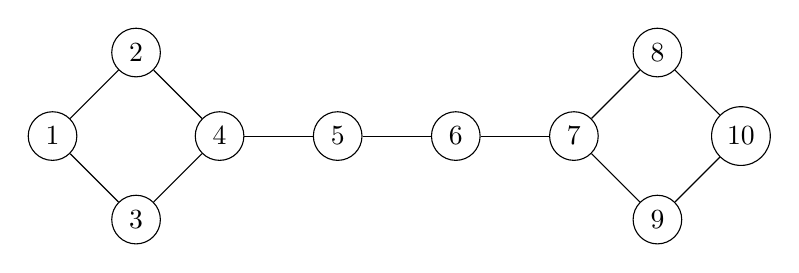
\begin{tikzpicture}[node distance={15mm}, main/.style = {draw, circle}] 
\node[main] (1) {1};
\node[main] (2) [above right of=1] {2};
\node[main] (3) [below right of=1] {3};
\node[main] (4) [below right of=2] {4};
\node[main] (5) [right of=4] {5};
\node[main] (6) [right of=5] {6};
\node[main] (7) [right of=6] {7};
\node[main] (8) [above right of=7] {8};
\node[main] (9) [below right of=7] {9};
\node[main] (10) [below right of=8] {10};
\draw[-] (1) -- (2);
\draw[-] (1) -- (3);
\draw[-] (2) -- (4);
\draw[-] (3) -- (4);
\draw[-] (4) -- (5);
\draw[-] (5) -- (6);
\draw[-] (7) -- (6);
\draw[-] (8) -- (7);
\draw[-] (9) -- (7);
\draw[-] (10) -- (8);
\draw[-] (10) -- (9);
\end{tikzpicture}
\caption{Dwudzielny graf nieskierowany.}
\end{figure}

\begin{figure}[H]
\centering
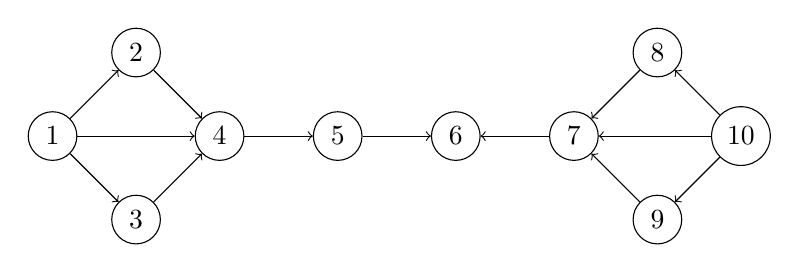
\begin{tikzpicture}[node distance={15mm}, main/.style = {draw, circle}] 
\node[main] (1) {1};
\node[main] (2) [above right of=1] {2};
\node[main] (3) [below right of=1] {3};
\node[main] (4) [below right of=2] {4};
\node[main] (5) [right of=4] {5};
\node[main] (6) [right of=5] {6};
\node[main] (7) [right of=6] {7};
\node[main] (8) [above right of=7] {8};
\node[main] (9) [below right of=7] {9};
\node[main] (10) [below right of=8] {10};
\draw[->] (1) -- (2);
\draw[->] (1) -- (3);
\draw[->] (1) -- (4);
\draw[->] (2) -- (4);
\draw[->] (3) -- (4);
\draw[->] (4) -- (5);
\draw[->] (5) -- (6);
\draw[->] (7) -- (6);
\draw[->] (8) -- (7);
\draw[->] (9) -- (7);
\draw[->] (10) -- (7);
\draw[->] (10) -- (8);
\draw[->] (10) -- (9);
\end{tikzpicture}
\caption{Niedwudzielny graf skierowany.}
\end{figure}

\begin{figure}[H]
\centering
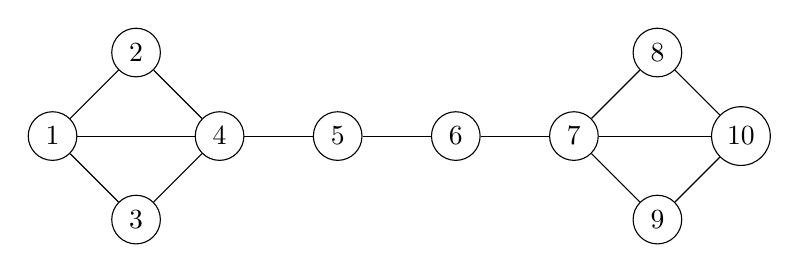
\begin{tikzpicture}[node distance={15mm}, main/.style = {draw, circle}] 
\node[main] (1) {1};
\node[main] (2) [above right of=1] {2};
\node[main] (3) [below right of=1] {3};
\node[main] (4) [below right of=2] {4};
\node[main] (5) [right of=4] {5};
\node[main] (6) [right of=5] {6};
\node[main] (7) [right of=6] {7};
\node[main] (8) [above right of=7] {8};
\node[main] (9) [below right of=7] {9};
\node[main] (10) [below right of=8] {10};
\draw[-] (1) -- (2);
\draw[-] (1) -- (3);
\draw[-] (1) -- (4);
\draw[-] (2) -- (4);
\draw[-] (3) -- (4);
\draw[-] (4) -- (5);
\draw[-] (5) -- (6);
\draw[-] (7) -- (6);
\draw[-] (8) -- (7);
\draw[-] (9) -- (7);
\draw[-] (10) -- (7);
\draw[-] (10) -- (8);
\draw[-] (10) -- (9);
\end{tikzpicture}
\caption{Niedwudzielny graf nieskierowany.}
\end{figure}

\subsection{Wyniki}
\begin{table}[H]
\begin{adjustbox}{center}
\begin{tabular}{|c|c|c|}
    \hline
    Graf & Skierowany & 2 zbiory wierzchołków\\
    \hline
    1 & TAK & [1 4 6 8 9], [2 3 5 7 10]\\
    \hline
    2 & NIE & [1 4 6 8 9], [2 3 5 7 10]\\
    \hline
    3 & TAK & Graf nie jest dwudzielny\\
    \hline
    4 & NIE & Graf nie jest dwudzielny\\
    \hline
\end{tabular}
\end{adjustbox}
\caption{Sprawdzenie dwudzielności grafu i podział na zbiory wierzchołków za pomocą BFS z kolorowaniem.}
\end{table}

\subsection{Czasy}
\begin{table}[H]
\begin{adjustbox}{center}
\begin{tabular}{|c|c|c|c|c|c|}
    \hline
    Plik & Skierowany & Dwudzielny & $|V|$ & $|E|$ & Czas [ns]\\
    \hline
    \textit{d4a-1.txt} & TAK & TAK & 16 & 24 & 13647\\
    \hline
    \textit{d4a-2.txt} & TAK & TAK & 100 & 180 & 66214\\
    \hline
    \textit{d4a-3.txt} & TAK & TAK & 1600 & 3120 & 1025125\\
    \hline
    \textit{d4a-4.txt} & TAK & TAK & 10000 & 19800 & 6286833\\
    \hline
    \textit{d4a-5.txt} & TAK & TAK & 160000 & 319200 & 101964833\\
    \hline
    \textit{d4a-6.txt} & TAK & TAK & 1000000 & 1998000 & 670709530\\
    \hline
    \textit{d4b-1.txt} & TAK & NIE & 16 & 25 & 12974\\
    \hline
    \textit{d4b-2.txt} & TAK & NIE & 100 & 181 & 59872\\
    \hline
    \textit{d4b-3.txt} & TAK & NIE & 1600 & 3121 & 898077\\
    \hline
    \textit{d4b-4.txt} & TAK & NIE & 10000 & 19801 & 5615172\\
    \hline
    \textit{d4b-5.txt} & TAK & NIE & 160000 & 319201 & 90784655\\
    \hline
    \textit{d4b-6.txt} & TAK & NIE & 1000000 & 1998001 & 580847940\\
    \hline
    \textit{u4a-1.txt} & NIE & TAK & 15 & 22 & 7592\\
    \hline
    \textit{u4a-2.txt} & NIE & TAK & 127 & 190 & 32867\\
    \hline
    \textit{u4a-3.txt} & NIE & TAK & 1023 & 1534 & 241987\\
    \hline
    \textit{u4a-4.txt} & NIE & TAK & 16383 & 24574 & 3956059\\
    \hline
    \textit{u4a-5.txt} & NIE & TAK & 131071 & 196606 & 31664039\\
    \hline
    \textit{u4a-6.txt} & NIE & TAK & 1048575 & 1572862 & 260706055\\
    \hline
    \textit{u4b-1.txt} & NIE & NIE & 15 & 22 & 6535\\
    \hline
    \textit{u4b-2.txt} & NIE & NIE & 127 & 190 & 25275\\
    \hline
    \textit{u4b-3.txt} & NIE & NIE & 1023 & 1534 & 182499\\
    \hline
    \textit{u4b-4.txt} & NIE & NIE & 16383 & 24574 & 3039818\\
    \hline
    \textit{u4b-5.txt} & NIE & NIE & 131071 & 196606 & 24284041\\
    \hline
    \textit{u4b-6.txt} & NIE & NIE & 1048575 & 1572862 & 200461039\\
    \hline
\end{tabular}
\end{adjustbox}
\caption{Porównanie czasów sprawdzania dwudzielności grafu za pomocą BFS z kolorowaniem dla danych z plików testowych.}
\end{table}

\end{document}